\documentclass[journal]{IEEEtran}
\usepackage[utf8]{inputenc}

\usepackage{graphicx}
%\usepackage[caption=false,font=footnotesize]{subfig}
\usepackage{url}
\usepackage{algorithmic}%
\usepackage{algorithm}%
\usepackage{multirow}%
\usepackage{xcolor}%
\usepackage{subcaption}%
\usepackage{placeins}%
\usepackage{circuitikz}%

\usepackage{url}
% Making the references and links clickable
\usepackage{hyperref}
\hypersetup{
    %colorlinks=false,
    pdfborder={0 0 0}
}

\usepackage{xcolor}
\newcommand{\todo}[1]{\textcolor{red}{#1}}
\newcommand{\mymotor}[2] % #1 = name , #2 = rotation angle
{\draw[thick,rotate=#2] (#1) circle (10pt)
 node[]{$\mathsf M$} 
++(-12pt,3pt)--++(0,-6pt) --++(2.5pt,0) ++(-2.8pt,6pt)-- ++(2.5pt,0pt);
\draw[thick,rotate=#2] (#1) ++(12pt,3pt)--++(0,-6pt) --++(-2.5pt,0) 
++(2.8pt,6pt)-- ++(-2.5pt,0pt);
}

\usepackage{fancyhdr}
\pagestyle{fancy}
\lhead{University of Brasília}
\rhead{\thepage}
\cfoot{Building an H Bridge}
\renewcommand{\headrulewidth}{0.4pt}
\renewcommand{\footrulewidth}{0.4pt}

\begin{document}
    \title{Building an H Bridge}
    
    \author{\IEEEauthorblockN{Bruno H. F. Macedo and
            Gabriel F. P. Araújo}
        \IEEEauthorblockA{
        % \\Laboratório de Automação e Robótica - LARA
        \\Universidade de Brasília - UnB\\
        Brasília - DF - Brasil}
        }
    
    \maketitle
    
    \begin{abstract}
        
        This work presents the design and implementation of an H bridge. The circuit was designed to be used with low power DC motors. This report will present as well the design, prototyping and manufacturing of the board.
                
    \end{abstract}
    
    \begin{IEEEkeywords}
        H bridge, robotics, electric circuits, electronic circuits.        
    \end{IEEEkeywords}
    
 
    \section{\textbf{Introduction}}\label{sec:1}
	DC motors are commonly used in robotics due to it's reduced size, light weight and easy velocity control~\cite{CHAPMAN}, avoiding the use of rectifiers or power inverters. In order to change the orientation of a DC motor, for instance, only the direction of the applied voltage needs to change.

	H bridges (see Figure~\ref{fig:bridge}) are simple electronic circuits used to enable a voltage to be applied across a motor in either direction. Despite it's simplicity H bridges might be used to accomplish more challenging tasks, such as stabilizing distributed energy sources~\cite{H-POWER-QUALITY} and improving power quality in electric vehicles~\cite{H-FILTERING}.

\begin{figure}[h]
\centering
% \begin{subfigure}[b]{0.4\textwidth}
	\centering%
	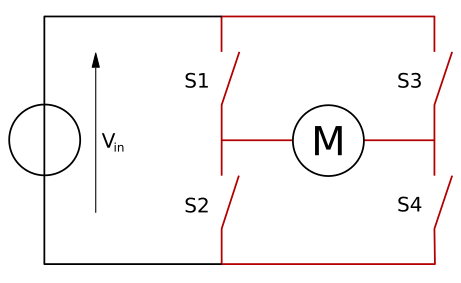
\includegraphics[height=.25\textwidth]{img/H_bridge.png}
	\caption[caption H Bridge]{H Bridge figure borrowed from wikipedia\protect\footnotemark.}
    \label{fig:bridge}%
% \end{subfigure}\hfill
\end{figure}
\footnotetext{\url{https://en.wikipedia.org/wiki/H_bridge}}

    \section{\textbf{Theory}}\label{sec:2}
    \todo{talk about the theory and the calculus. What theory? what calculus?}

    \section{\textbf{Simulation}}\label{sec:3}

\begin{figure*}
\centering
	\begin{subfigure}{.45\textwidth}
    \centering
    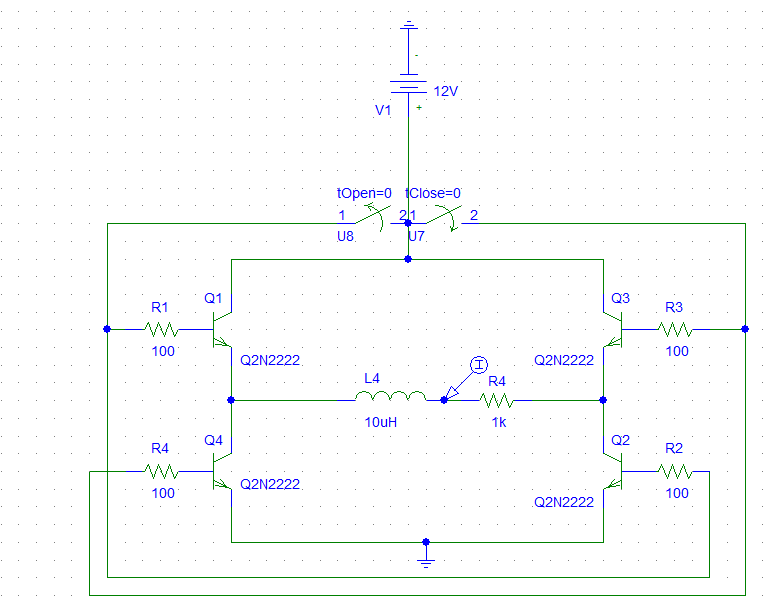
\includegraphics[width=\linewidth]{img/schem_pspice.png}
    \caption{Schematic on PSpice program.}\label{fig:schem_pspice}%
    \end{subfigure}    
    \begin{subfigure}{.45\textwidth}
    ~
    \centering
    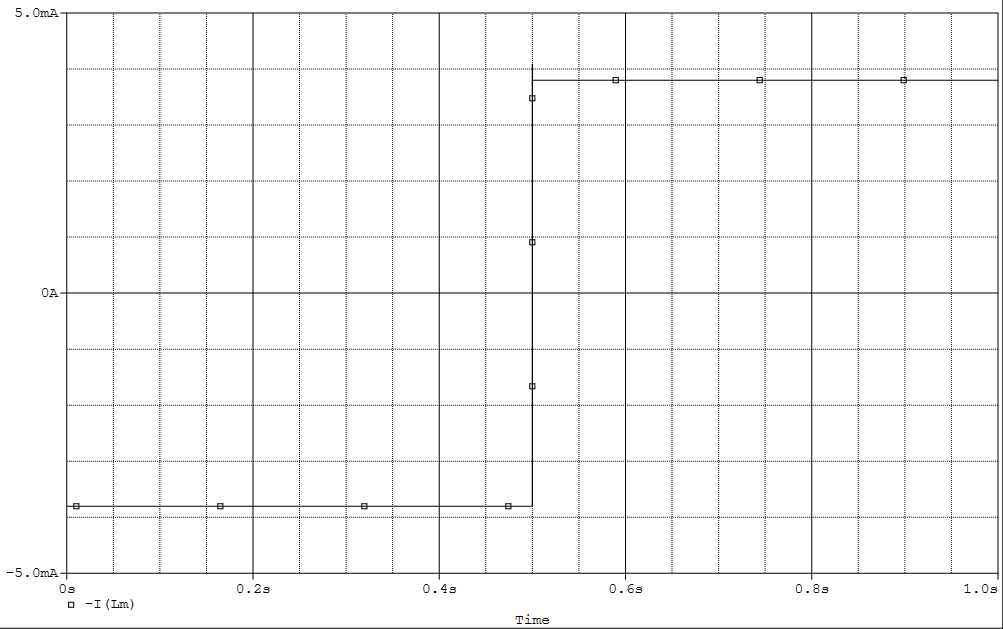
\includegraphics[width=\linewidth, height=6.4cm]{img/plot.png}
    \caption{Current x Time} \label{fig:plot_ponteh}
	\end{subfigure}
	\caption{Simulation analysis.}
	
\end{figure*}

    The circuit design was simulated using PSpice software distributed by OrCAD. The circuit shown in Figure~\ref{fig:schem} was reproduced in PSpice (see Figure \ref{fig:schem_pspice}). The software does not support the transistor model used in the actual implementation, the TIP31C, instead the Q2N2222 was used to replace it given they are very similar, only the maximum supported values for voltages change. The value of all transistors base resistances was set to $100\:\Omega$. The DC motor simplified equivalent circuit is an inductor and a resistor~\cite{CHAPMAN}. The U8 and U7 times were set to $500\; ms$.\newline
    The motor used in the tests are the one included on the Magician Chassis\footnote{https://www.sparkfun.com/products/retired/12866} by Sparkfun, they have the following characteristics:
    \begin{itemize}
        \item Max Motor Voltage: 6 VDC;
        \item No Load Speed: $90\pm10$ rpm;
        \item No Load Current:190 mA (max.250 mA);
        \item Torque: 800 gf.cm;
    \end{itemize}
	Finally a transient analysis over the circuit was made and the current flowing through the motor is plotted in Figure~\ref{fig:plot_ponteh}. The simulated circuit behavior is exactly the expected, when Q1 and Q2 are activated the current flows in the positive direction, in opposition to Q3 and Q4 active which results in a negative current flow.
	

\begin{figure}[htp!]
\begin{center}
\begin{circuitikz} %\label{sec:1}
    \draw (2,0) node[npn](q1) at (2,0){}
    (q1.E) node[npn](q4) at (2,-1.55){}
    (q1.E) -- (q4.C);
    \draw (-0.55,0) to[R] (q1.B){};
    \draw (-0.55,-1.55) to[R] (q4.B){};
    \draw (5,0) node[npn,xscale=-1](q3) at (4,0){}
    (q3.E) node[npn,xscale=-1](q2) at (4,-1.55){}
    (q3.E) -- (q2.C)
    (q1.C) -- (q3.C)
    (q4.E) -- (q2.E);
    \draw (3,-2.55) node[ground](gnd){}
    (q2.E) |- (gnd);
    \draw (q3.B)  to[R] (6,0);
    \draw (q2.B) to[R] (6,-1.55);
    % \draw (q1.E) node[elmech]{M}) (q3.E);
    \draw (-0.55,0) -- (-1.0,0) node[circ]{} -- (-1.0,-4) -- (7,-4) -- (7,-1.55) -- (6,-1.55);
    \draw (-0.55,-1.55) -- (-0.80,-1.55) -- (-0.8,-3.5) --(6.5,-3.5) -- (6.5,0) node[circ]{} -- (6,0);
    \draw (3,2) node[spdt,xscale=-1] (s1){}
    (s1.in) |- node[circ]{} (q1.C)
    (s1.out 1) |- (3.5,2.5) |- (7,2.5) |- (6,0)
    (s1.out 2) |- (-1,1.685) |- (-1,0);
    \draw (q1.E) to[sV, color=white, name=M1] (q3.E);
    \mymotor{M1}{0}
    \draw (q2.E) node[circ]{} |- (7.5,-2.31) to[battery] (7.5,1) |- (4,1) |- node[circ]{} (q3.C);
    % \draw (q1.C) --++(0,0.5) node[vcc]{+4.5\,\textnormal{V}};
    % \mymotor{M}{0}
    % \draw (q1.B) -- to[R=100<\ohm>]{};
    % \draw (0,0) node[npn](npn) at (0,0){};
\end{circuitikz}
\caption{H Bridge}\label{fig:schem}%
\end{center}
\end{figure}


    \section{\textbf{Manufacturing}}\label{sec:4}
    \todo{Show the fritzing environment, the schematics, board design and board manufacturing}
	As the simulation (see Section~\ref{sec:3}) proved that the designed circuit works as intended the physical components were assembled in a protoboard for further testing and validation before the final manufacturing \todo{complete with relevant information about final board}. Figure\todo{INSERT AND REF PROPOER PROTOBOARD FIGURE} shows the circuit properly assembled. This circuit's evaluation will be further discussed in Section~\ref{sec:5}.
	
	\todo{TALK ABOUT CIRCUIT PRINTING}
	
    \section{\textbf{Evaluation}}\label{sec:5}

	First of all the breadboard circuit (Figure~\ref{fig:proto_h}) was tested using a multimeter to ensure it's proper functionality. With Q1 and Q2 activated the voltage measured across the motor was $3.5\;V$, for future analysis this situation (Q1 and Q2 active) will be called S1. With Q3 and Q4 activated the voltage measured was $-2.6\;V$, this will be the S2 situation. The polarity inversion was accomplished, however the magnitude for both cases which was expected to be equal was in fact different. A slightly tension drop occurred when the current flew backwards. One important thing to mention is that when the transistor is turned off (base voltage = 0) it's output is not exactly equals zero, it shows a remainder voltage of $0.6\;V$ however this tension is not enough to move the motor.
	
	Despite the previous mentioned discrepancy, which solution will be discussed later on the circuit performed as intentioned therefore the motor was plugged into the circuit. For S1 the motor spun in the counterclockwise direction. On the other hand for S2 it spun clockwise slightly slower, as a result of the voltage drop previous mentioned.
	
	Finally with the printed circuit board in hands the tension across the output pins were once again measured with a voltmeter. In case S1 the voltage showed up to be $3.6\;V$ which is equal to the breadboard circuit, the same occurred for S2. As the PCB performed exactly as the breadboard circuit the motor was connected and the final configuration version 1 was achieved.
	
	In order to achieve a better performance and eliminate the previous mentioned tension drop for S2 this configuration needed to change a bit. A possible cause for this issue was a remaining current when the transistor should be turned off. Hence four resistors were added between the transistor's base resistor and the ground node (see Figure~\ref{fig:h_schem_v2}. The intention of this change is to force any remaining current flows to the ground node.
	
	The final configuration version 2 filled the expectations. For S1 case the tension across the motor was $3.84\;V$. And now for S2 case the tension showed to be $-3.78\;V$ which result in equal spin velocity for both cases.
	
\begin{figure}[b]
\centering
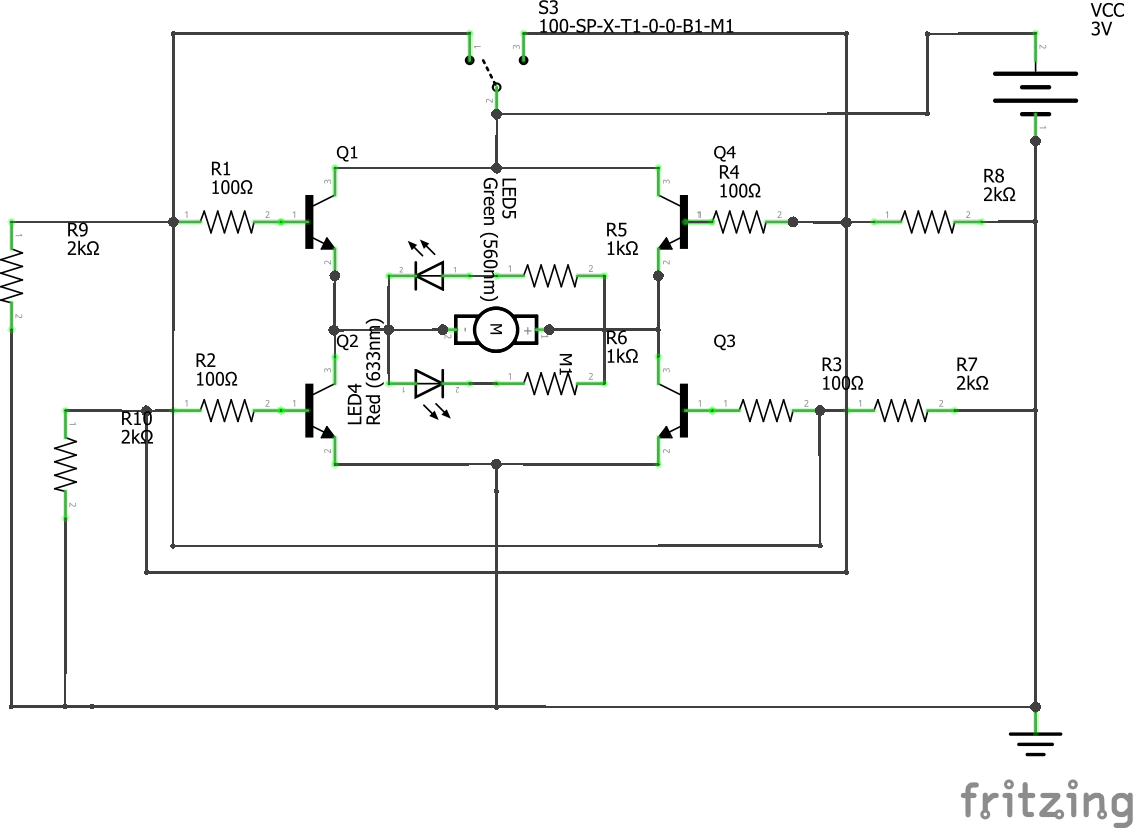
\includegraphics[width=\columnwidth]{img/ponteH_schem_new.png}
\caption{Final configuration version 2 schematic.}
\label{fig:h_schem_v2}
\end{figure}


    \section{\textbf{Conclusion}}\label{sec:6}
This paper demonstrated how the concepts acquired through the course could be brought in real world applications like a simplistic H bridge circuit being able to control the direction of a moving robot.

The built H bridge proved to be an efficient device for controlling the speed of a low power DC motor. It is, in general, a simple circuit with wide usage among robotics applications due to it's versatility. A more elaborate approach might make use of PWM with H bridge for additional control over the motor's velocity.

    % \input{Future_Works}

    \section{Acknowledgments} % (fold)
    \label{sec:acknowledgments}
        The authors would like to thank the members of the laboratory LARA by given space, time and tips in addition to borrowing the milling machine. An especial thanks to Miguel Eduardo and Breno Ferreira, both PhD candidates at LARA, for guiding the authors through soldering and printing skills.
    % section acknowledgements (end)
    
    %\nocite{*}
    \bibliographystyle{IEEEtran}
    \bibliography{Bibliography}
    % \toDo{Adequar as referências ao padrão do IEEE: \url{http://www.ieee.org/documents/ieeecitationref.pdf}. Quando
    % há 3 ou mais autores colocar et al.}
    
    
    
\end{document}
